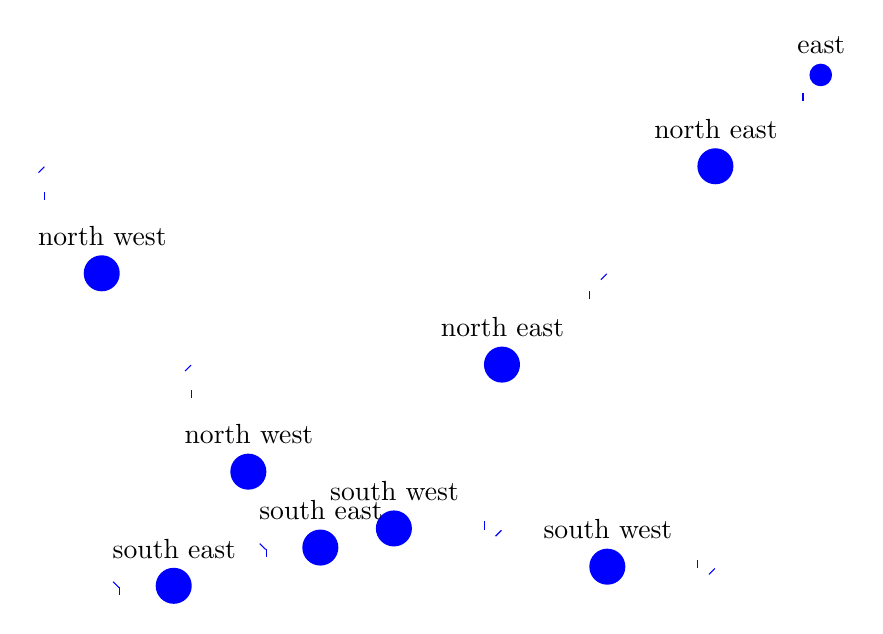
\begin{tikzpicture}
\hiddenneuron{blue}{0/0, 0/-1, 1/-1, -1/-1};
\hiddenneuron[green]{45}{0/0, 0/-1, 1/-1, -1/-1};
\hiddenneuron[red]{-45}{0/0, 0/-1, 1/-1, -1/-1};

\node[blue,circle,fill=blue,inner sep=0pt,minimum size=.7em,label={south west}] 
    (w1) at (current bounding box.south east) {$w_1$};
\draw[dashed,blue] (current bounding box.south east) ++(45:.3) -- ++(90:.2);
\draw[dashed,blue] (current bounding box.south east) ++(45:.3) -- ++(225:.2);

\node[blue,circle,fill=blue,inner sep=0pt,minimum size=.7em,label={south east}] 
    (w2) at (current bounding box.south west) {$w_2$};
\draw[dashed,blue] (current bounding box.south west) ++(45:.3) -- ++(270:.2);
\draw[dashed,blue] (current bounding box.south west) ++(45:.3) -- ++(135:.2);

\node[blue,circle,fill=blue,inner sep=0pt,minimum size=.7em,label={north west}] 
    (w3) at (current bounding box.north west) {$w_3$};
\draw[dashed,blue] (current bounding box.north west) ++(45:.3) -- ++(90:.2);
\draw[dashed,blue] (current bounding box.north west) ++(45:.3) -- ++(225:.2);

\node[blue,circle,fill=blue,inner sep=0pt,minimum size=.7em,label={north east}] 
    (w4) at (current bounding box.north east) {$w_4$};
\draw[dashed,blue] (current bounding box.north east) ++(45:.3) -- ++(-90:.2);
\draw[dashed,blue] (current bounding box.north east) ++(45:.3) -- ++(-135:.2);

\node[blue,circle,fill=blue,inner sep=0pt,minimum size=.7em,label={south west}] 
    (w1) at (current bounding box.south east) {$w_1$};
\draw[dashed,blue] (current bounding box.south east) ++(45:.3) -- ++(90:.2);
\draw[dashed,blue] (current bounding box.south east) ++(45:.3) -- ++(225:.2);

\node[blue,circle,fill=blue,inner sep=0pt,minimum size=.7em,label={south east}] 
    (w2) at (current bounding box.south west) {$w_2$};
\draw[dashed,blue] (current bounding box.south west) ++(45:.3) -- ++(270:.2);
\draw[dashed,blue] (current bounding box.south west) ++(45:.3) -- ++(135:.2);

\node[blue,circle,fill=blue,inner sep=0pt,minimum size=.7em,label={north west}] 
    (w3) at (current bounding box.north west) {$w_3$};
\draw[dashed,blue] (current bounding box.north west) ++(45:.3) -- ++(90:.2);
\draw[dashed,blue] (current bounding box.north west) ++(45:.3) -- ++(225:.2);

\node[blue,circle,fill=blue,inner sep=0pt,minimum size=.7em,label={north east}] 
    (w4) at (current bounding box.north east) {$w_4$};
\draw[dashed,blue] (current bounding box.north east) ++(45:.3) -- ++(-90:.2);
\draw[dashed,blue] (current bounding box.north east) ++(45:.3) -- ++(-135:.2);
\node[blue,circle,fill=blue,inner sep=0pt,minimum size=.7em,label={east}] 
    (b) at (current bounding box.north east) {$b$};
\end{tikzpicture}